\section{Versuchsbeschreibug}
\label{section:Versuchsbeschreibung}
%
\begin{figure}[!h]
		\centering
		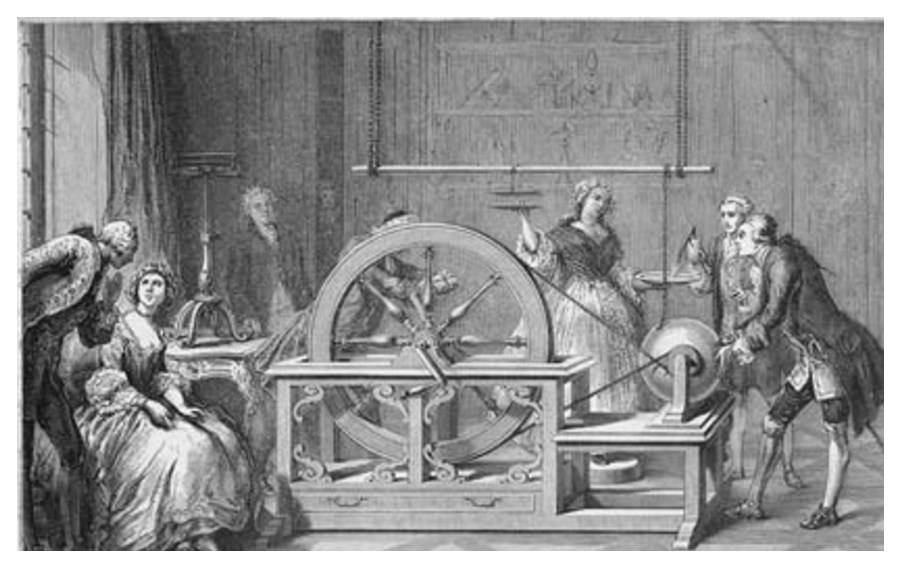
\includegraphics[width=0.5\textwidth]{Abbildungen/Beispielbild_Versuchsaufbau.eps}
		\caption{Foto oder Skizze des Versuchsaufbaus}
		\label{fig:BspVers}
\end{figure}
%
Werden Textpassagen (wie z.B. Definitionen) wörtlich übernommen, dann müssen diese auch durch eine Quellenangabe kenntlich gemacht werden. Die dazugehörigen Quellen werden im Literaturverzeichnis aufgeführt.\\

Die verwendeten Messgeräte und deren Genauigkeit sind als Auflistung oder tabellarisch darzustellen.\\

Beispiel:
%
\begin{itemize}
\item Laser-Umdrehungsmesser Conrad DT2234C, Auflösung 1 1/min $\pm$1 Digit
\end{itemize}
%
